\newpage
\section{The Evolution of Sustainable Logistics}
\begin{figure}[!h]
    \centering
    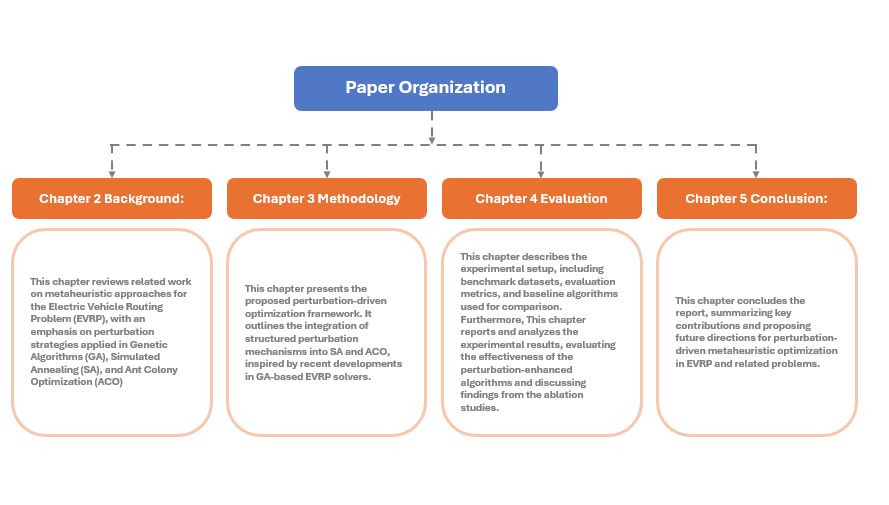
\includegraphics[width=1\linewidth]{image/1/paper_structure1.png}
    \caption{Background Structure}
    \label{fig:bg}
\end{figure}
\subsection{Environmental Concerns and CO\textsubscript{2} Emissions}

Climate change, driven primarily by the escalation of greenhouse gas emissions, has emerged as one of the most critical global challenges of the 21\textsuperscript{st} century~\cite{mccarthy2010climate}.  
The transportation sector is a major contributor, responsible for approximately 24\% of global direct CO\textsubscript{2} emissions from fuel combustion~\cite{edenhofer2015climate}.  
This significant environmental footprint has intensified pressure on governments, industries, and researchers to pursue sustainable alternatives to conventional transportation practices.

In particular, urban freight transport—dominated by logistics and delivery services—plays a disproportionate role in exacerbating air pollution within cities.  
As urbanization accelerates and e-commerce demand surges, the need for efficient yet environmentally sustainable logistics solutions has become increasingly urgent.


\subsection{Logistics Sector's Shift Towards Electrification}

In response to escalating environmental concerns and increasing regulatory pressures, the logistics sector is undergoing a fundamental transformation toward more sustainable practices.  
One of the most prominent trends is the electrification of vehicle fleets, with major logistics companies such as FedEx, UPS, and DHL making substantial investments in EVs to reduce their carbon footprint~\cite{zuo2019new, soleimani2018collection}.

EVs offer several advantages over their internal combustion engine counterparts, including zero tailpipe emissions, higher energy efficiency, and lower maintenance costs.  
These benefits align closely with corporate sustainability objectives and the growing consumer demand for greener supply chains.  
Nevertheless, integrating EVs into existing logistics operations introduces significant challenges, particularly regarding limited driving range, battery degradation, and the need for extensive charging infrastructure.


\subsection{Importance of Optimizing EV-Based Delivery Routes}

While the deployment of EVs represents a critical step toward sustainable logistics, their successful integration depends heavily on addressing their unique operational constraints.  
Unlike conventional internal combustion engine vehicles, EVs require meticulous route planning to ensure that delivery schedules are met without depleting battery reserves.  
Factors such as energy consumption rates, charging station availability, and vehicle load capacities must all be carefully considered in the routing process.

Optimizing EV-based delivery routes is therefore essential to fully realizing the environmental and economic benefits of fleet electrification.  
Effective routing minimizes the total distance traveled, reduces the frequency and duration of charging stops, and maximizes vehicle utilization, thereby enhancing the overall efficiency and sustainability of logistics operations.  
This necessity has given rise to the EVRP, a complex extension of the classical Vehicle Routing Problem, specifically tailored to account for the operational characteristics and limitations of EVs.

Addressing the EVRP through advanced optimization techniques not only reduces operational costs and environmental impact but also plays a vital role in accelerating the broader adoption of electric mobility within the logistics sector.



\section{From VRP to EVRP: Problem Transformation}

The Vehicle Routing Problem (VRP) is a classical combinatorial optimization problem concerned with determining optimal routes for a fleet of vehicles to service a set of customers from a central depot.  
Each customer must be visited exactly once, and the total travel distance or cost must be minimized, subject to constraints such as vehicle load capacity and maximum route duration.

While extensively studied, the classical VRP does not account for energy-related limitations.  
As electric vehicles (EVs) increasingly replace traditional internal combustion engine (ICE) vehicles, the routing paradigm must be adapted to accommodate additional constraints such as battery capacity, energy consumption per route segment, and the availability and location of charging stations.  
This gives rise to the Electric Vehicle Routing Problem (EVRP), which generalizes the VRP by embedding energy-awareness into the model.

Formally, let $G = (V, E)$ denote a complete directed graph, where $V = \{v_0, v_1, \dots, v_n\}$ represents the set of nodes, with $v_0$ corresponding to the depot and $\{v_1, \dots, v_n\}$ the customer locations.  
Each edge $(i, j) \in E$ is associated with a travel cost $c_{ij}$ and an energy consumption value $e_{ij}$.  
Each EV has a battery capacity $Q$ and may recharge at designated charging stations $R \subset V$.

A feasible route $r = \{v_0, v_{i_1}, v_{i_2}, \dots, v_{i_k}, v_0\}$ must satisfy the following constraints:

\begin{itemize}
    \item \textbf{Visit constraint}: Each customer node $v_i \in V \setminus \{v_0\}$ must be visited exactly once.
    \item \textbf{Capacity constraint}: The total demand served along a route must not exceed the vehicle's load capacity.
    \item \textbf{Energy constraint}: The cumulative energy consumption along any route segment between recharges must not exceed the battery capacity $Q$:
    \[
        \sum_{(i, j) \in r'} e_{ij} \leq Q
    \]
    where $r'$ denotes any sub-route between two recharge points.
    \item \textbf{Recharge feasibility}: Vehicles may recharge at designated nodes $v_j \in R$, where the battery is fully replenished.
\end{itemize}

Compared to the classical VRP, the inclusion of energy-aware constraints significantly increases the solution space complexity.  
Routing algorithms must not only determine customer visiting sequences but also strategically plan recharge stops, optimize energy usage, and account for additional factors such as vehicle load and terrain elevation.

Moreover, EVRP introduces the possibility of infeasible partial solutions—routes that may be cost-optimal but invalid due to battery depletion before reaching a charging station.  
This necessitates the integration of robust feasibility checking and solution repair mechanisms within optimization procedures.

As an extension of the VRP, the EVRP additionally requires the planning of charging station visits alongside customer servicing (Fig.~\ref{fig:vs}).  
Since the classical VRP is already known to be NP-hard, the EVRP, as its generalization, remains strongly NP-hard.  
Furthermore, the incorporation of energy and recharge constraints, as outlined above, renders the problem even more challenging to solve.

\begin{figure}
    \centering
    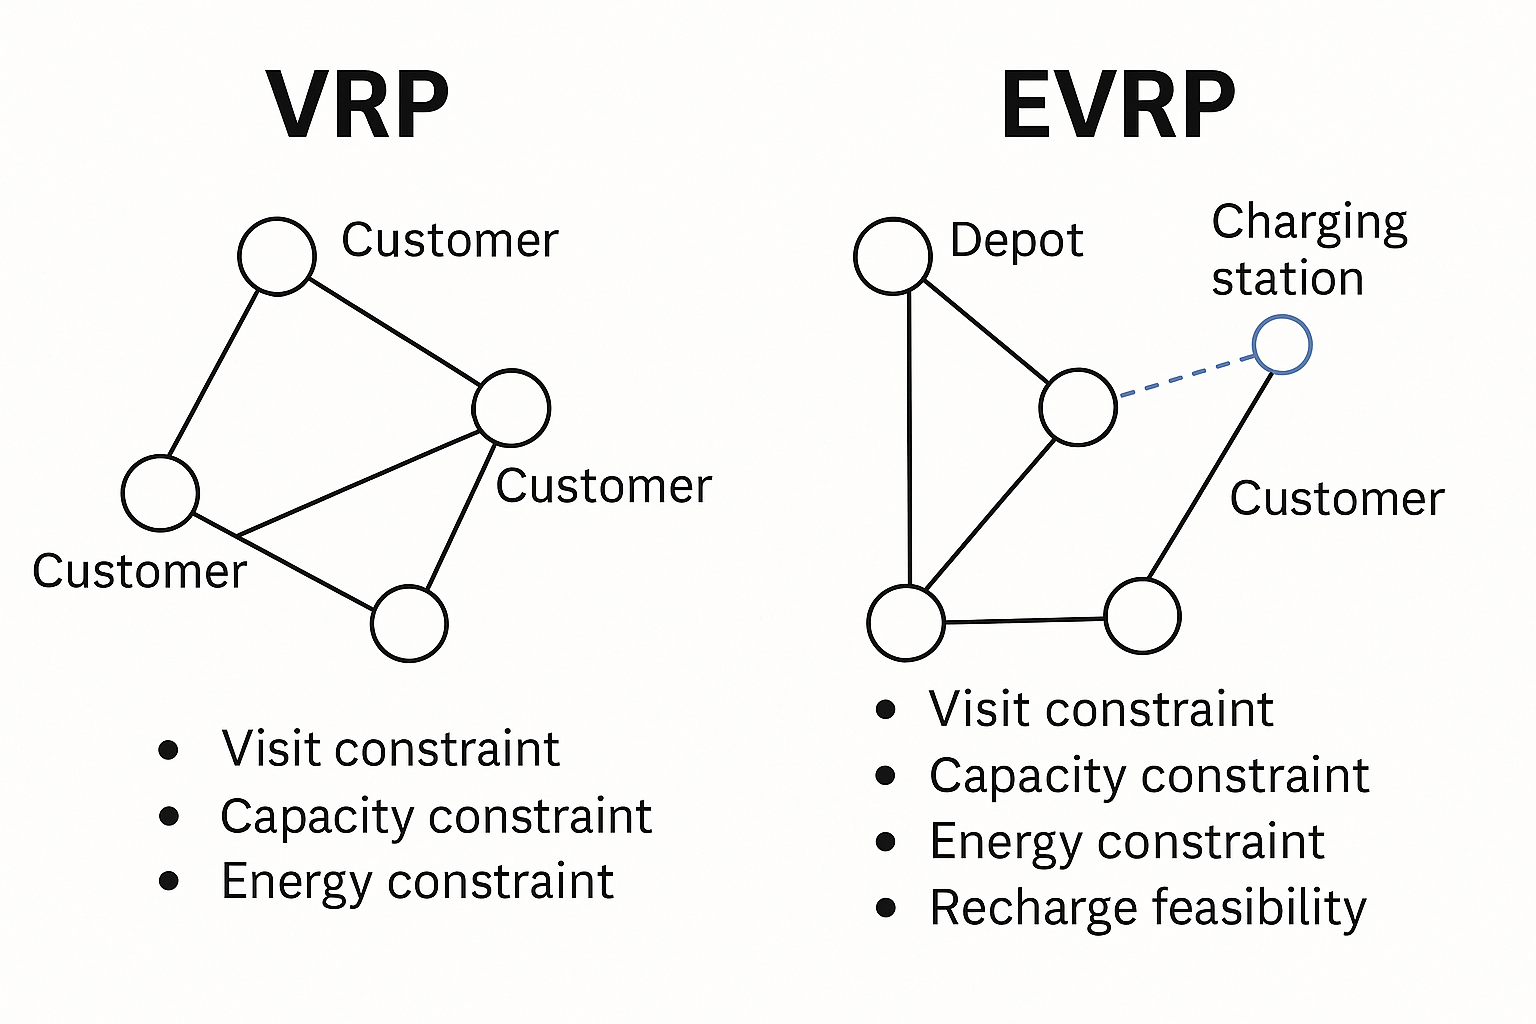
\includegraphics[width=1\linewidth]{image/2/Logistics Optimization_ VRP vs EVRP.png}
    \caption{VRP vs. EVRP}
    \label{fig:vs}
\end{figure}


\subsection{Problem Definition of the Electric Vehicle Routing Problem}

The Electric Vehicle Routing Problem involves determining a set of vehicle routes, where each route serves a subset of customer nodes and must both start and end at a designated depot~\cite{schiffer2017electric}.  
The primary objective is to optimize route planning for electric vehicles by minimizing a given cost function, typically the total travel distance, while satisfying operational constraints associated with vehicle limitations.

The EVRP is based on the following key assumptions~\cite{kucukoglu2021electric}:
\begin{itemize}
    \item Each route begins and ends at the depot.
    \item Each customer node is visited exactly once by exactly one vehicle.
    \item Vehicles are allowed to visit charging stations en route to replenish their battery.
    \item Multiple vehicles may use the same charging station without restriction.
    \item The distances between all nodes and the locations of charging stations are known and fixed.
    \item The battery level of each vehicle must remain within the bounds of zero and its maximum capacity at all times during operation.
    \item After visiting a charging station, the vehicle's battery is assumed to be fully recharged.
\end{itemize}

Compared to the classical Vehicle Routing Problem, the EVRP introduces additional complexities by explicitly modeling energy constraints, necessitating strategic planning of charging station visits alongside customer servicing.

\subsubsection{Current Classifications of EVRP Models}

\paragraph{Based on Objective Functions}

Existing EVRP models can be categorized according to their primary optimization objectives.  
A large body of work, including studies by Chen et al.~\cite{chen2016electric}, Cubides et al.~\cite{cubides2019electric}, Catay and Keskin~\cite{ccatay2017impact}, and Ding et al.~\cite{ding2015conflict}, focuses on minimizing the total travel distance, reflecting the traditional VRP objective.

Other studies, such as those by Abdulaal et al.~\cite{abdulaal2016solving}, Ceselli et al.~\cite{ceselli2021branch}, and Felipe et al.~\cite{felipe2014heuristic}, prioritize minimizing total charging cost or total charging time, acknowledging the practical impact of prolonged recharging in EV operations.

Additionally, a third group of research, including the works of Abdallah et al.~\cite{abdallah2020electric}, Barco et al.~\cite{barco2017optimal}, and Basso et al.~\cite{basso2019energy, basso2021electric}, adopts total energy consumption as the main optimization objective, reflecting the growing importance of energy efficiency in sustainable logistics.

\paragraph{EVRP Constraints}

Compared to the classical Vehicle Routing Problem, the Electric Vehicle Routing Problem introduces additional constraints, with energy management during recharging being a particularly critical aspect.  
Charging constraints in EVRP models are generally classified into two categories: full charging and partial charging strategies.

Under the \textbf{full charging} assumption, vehicles must leave charging stations with fully replenished batteries.  
This simplifies energy tracking but may increase charging times and lead to potential inefficiencies.  
Representative studies adopting this assumption include Ghobadi et al.~\cite{ghobadi2021multi}, Goeke and Schneider~\cite{goeke2015routing}, Granada-Echeverri et al.~\cite{granada2020electric}, Hiermann et al.~\cite{hiermann2016electric}, Jia et al.~\cite{jia2021bilevel}, and Keskin et al.~\cite{keskin2016partial}.

Conversely, \textbf{partial charging} strategies allow vehicles to leave charging stations with incomplete recharges, depending on operational needs and time constraints.  
Partial charging offers greater routing flexibility and can enhance overall system efficiency, especially under nonlinear charging dynamics or tight delivery windows.  
Notable works adopting this approach include Bruglieri et al.~\cite{bruglieri2017three}, Futalef et al.~\cite{futalef2020evolutionary}, Karakatic~\cite{karakativc2021optimizing}, Kouider et al.~\cite{kouider2018constructive}, and Lee et al.~\cite{lee2021exact}.

In summary, the choice of optimization objective and charging strategy significantly influences EVRP model design, solution complexity, and applicability to real-world logistics scenarios.


\section{Approaches to Solving EVRP}

As an extension of the classical VRP, which is known to be NP-hard, the EVRP is similarly classified as a strongly NP-hard problem~\cite{desaulniers2016exact,ferro2018optimization,roberti2016electric}.  
Solving the EVRP requires algorithms capable of addressing not only the underlying combinatorial complexity but also the additional operational constraints introduced by limited battery capacity and recharging requirements.  
Over the years, researchers have proposed a wide range of solution techniques, which can be broadly categorized into three main groups: exact methods, heuristic strategies, and metaheuristic frameworks.

\subsection{Exact Methods for Solving EVRP}

Exact methods aim to compute globally optimal solutions by formulating the EVRP within a rigorous mathematical programming framework.  
Among these, Mixed Integer Programming (MIP) models are most commonly employed, where routing decisions, energy consumption tracking, and recharging operations are represented by a combination of binary and continuous variables.  
However, the integration of energy constraints greatly enlarges the solution space, making pure MIP formulations computationally impractical for large-scale instances.

To enhance tractability, advanced strategies such as Branch-and-Bound, Branch-and-Cut, and Branch-and-Price have been developed.  
Branch-and-Cut approaches strengthen linear programming relaxations via the addition of valid inequalities, while Branch-and-Price utilizes dynamic column generation to manage exponentially large route sets more efficiently.  
Hybrid Branch-Price-and-Cut frameworks, which combine these two ideas, currently represent the state-of-the-art among exact EVRP solvers.  
Moreover, Set Partitioning formulations are sometimes adopted, particularly when feasible energy-valid paths can be precomputed.

Notable examples of exact solution approaches include Tahami et al.~\cite{tahami2020exact}, who applied a Branch-and-Bound algorithm to standard EVRP instances, and Lee et al.~\cite{lee2021exact}, who developed a Branch-and-Price method to optimally solve EVRP variants involving nonlinear charging time models.

Despite their theoretical rigor and ability to guarantee optimality, exact methods face severe scalability challenges.  
Solution times increase exponentially with the number of customers, charging stations, or additional modeling complexities such as partial charging, heterogeneous fleets, or time windows.  
Consequently, exact methods are primarily restricted to small- or medium-sized instances and are mainly used for benchmarking heuristic and metaheuristic approaches.

In addition to bespoke academic solvers, commercial optimization software such as CPLEX~\cite{hulagu2019multiple,keskin2019electric} and GUROBI~\cite{moghaddam2015partially,schiffer2017electric} have also been employed for solving specific EVRP formulations.  
However, even with these powerful solvers, handling large-scale EVRP instances remains a substantial computational challenge.



\subsection{Heuristic Methods for Solving EVRP}

Heuristic methods for solving the Electric Vehicle Routing Problem (EVRP) are based on empirical strategies designed to quickly generate feasible, though not necessarily optimal, solutions.  
They are generally classified into two categories: constructive heuristics and improvement heuristics.

Constructive heuristics, such as nearest neighbor and savings-based approaches, incrementally build a feasible solution by inserting customer nodes and charging stations while satisfying energy and capacity constraints.  
Greedy Recharging Heuristic (GRH) strategies further extend these methods by incorporating energy-aware selection criteria, considering not only travel distance but also residual battery levels and proximity to charging infrastructure~\cite{felipe2014heuristic,schiffer2018adaptive,schneider2014electric}.

Improvement heuristics focus on enhancing an existing solution through local search operations.  
Common neighborhood operators include swap, relocate, and 2-opt or 3-opt moves, which aim to reduce total route cost while maintaining feasibility with respect to energy constraints.  
To address constraint violations arising during local search, specialized repair mechanisms are often integrated into the optimization process.

An alternative to heuristic-based charging station insertion is the use of forward labeling algorithms based on dynamic programming principles.  
Labeling methods systematically extend partial routes from the depot, inserting charging stations as necessary to maintain feasibility concerning battery capacity and time windows.  
By progressively constructing feasible paths, these algorithms can identify optimal recharge patterns for a given customer sequence.  
Although labeling algorithms are generally more computationally intensive than heuristic insertion methods, they often yield higher-quality solutions when computational resources permit.  
The charging station insertion problem, closely related to the resource-constrained shortest path problem, is also known to be strongly NP-hard~\cite{hiermann2016electric}.

Despite their computational efficiency, heuristic methods have inherent limitations.  
They are prone to premature convergence to suboptimal solutions, particularly in large-scale or highly constrained instances, and their manually crafted rules may lack adaptability to different EVRP variants, such as models with partial recharging or heterogeneous fleets.

Nevertheless, due to their low computational overhead, heuristic approaches remain valuable for quickly producing high-quality initial solutions, providing effective warm starts for metaheuristic algorithms, and serving as baselines for comparative evaluations.

\subsection{Metaheuristic Methods}

Metaheuristics are high-level strategies that guide local or global search procedures using problem-agnostic frameworks. They strike a balance between solution quality and scalability, making them particularly suitable for real-world EVRP instances.

\paragraph{Genetic Algorithms}

Genetic Algorithms (GAs) are population-based metaheuristic optimization techniques inspired by the principles of natural evolution. In the context of EVRP, GAs evolve a population of candidate solutions (routes) over successive generations to progressively enhance solution quality while satisfying energy constraints~\cite{abdallah2020electric}.

At each generation, the algorithm maintains a population of individuals, where each individual represents a feasible or partially feasible sequence of customer visits and recharging decisions. The evolutionary process consists of three primary operators: selection, crossover, and mutation.

\textbf{Selection:} A subset of parent solutions is selected from the current population based on fitness, typically evaluated according to the total route cost or energy consumption. Common selection strategies include tournament selection and roulette-wheel selection.

\textbf{Crossover:} Two parent solutions are combined to produce offspring by exchanging subsequences of customer visits and recharge decisions. In EVRP-specific adaptations, crossover operators are often designed to preserve energy-feasible segments or prioritize recharging station placements.

\textbf{Mutation:} Offspring solutions undergo random perturbations to maintain diversity and avoid premature convergence. Mutation operations may include swapping two customer nodes, inserting or removing a recharge station, or reversing a subsequence, with energy constraints checked or repaired as necessary.

After crossover and mutation, a new population is generated. The best-performing individuals may be retained through elitism to ensure steady improvement. The evolutionary cycle continues until a predefined stopping criterion is met, such as a maximum number of generations or convergence of solution quality.

Throughout the search process, energy feasibility checking and repair heuristics are integrated to ensure that candidate solutions remain valid under EVRP-specific operational constraints~\cite{abdulaal2016solving}.

\begin{algorithm}[H]
\caption{Genetic Algorithm for EVRP}
\begin{algorithmic}[1]
\State Initialize population $P$ with $N$ feasible or partially feasible routes
\While{stopping criterion not met}
    \ForAll{individuals in $P$}
        \State Evaluate fitness
    \EndFor
    \State Select parent solutions based on fitness
    \State Apply crossover to generate offspring
    \State Apply mutation to offspring
    \ForAll{offspring}
        \If{infeasible}
            \State Repair solution
        \EndIf
    \EndFor
    \State Form new population $P'$ by selecting the best individuals (elitism)
    \State $P \gets P'$
\EndWhile
\State \Return Best solution found
\end{algorithmic}
\end{algorithm}

Genetic Algorithms provide a flexible and robust framework for exploring the complex and multimodal solution space of EVRP, effectively balancing exploration and exploitation through stochastic evolutionary operators.


\paragraph{Simulated Annealing}

Simulated Annealing (SA) is a single-solution-based metaheuristic inspired by the physical annealing process in metallurgy, where controlled cooling enables a material to reach a low-energy crystalline structure. In the context of EVRP, SA explores the solution space by iteratively perturbing a current solution and probabilistically accepting candidate solutions based on both solution quality and a dynamically decreasing temperature parameter~\cite{erdougdu2020distance}.

At each iteration, the current solution is modified using a neighborhood operator to generate a new candidate solution. The acceptance decision for the new solution depends on a probability function that considers both the change in objective function value and the current temperature. Worse solutions may be accepted with a certain probability, allowing the algorithm to escape local minima during the early stages of the search.

Initially, the temperature is set to a high value to encourage exploration across the solution landscape. As the search progresses, the temperature is gradually reduced according to a cooling schedule, typically following a geometric decay pattern, where each new temperature is a fraction of the previous one. The rate of temperature decrease controls the balance between exploration and exploitation.

Energy feasibility is maintained during the generation of neighbor solutions, with repair heuristics applied when necessary to ensure that battery constraints and recharge station feasibility are satisfied. Typical neighborhood moves in EVRP-specific SA implementations include customer swap, insertion or removal of recharge stops, subsequence reversal, and reassignment of charging stations.

The algorithm continues until a predefined termination condition is met, such as reaching a minimum temperature threshold or a maximum number of iterations. By accepting uphill moves early in the search and gradually reducing the acceptance probability, Simulated Annealing effectively balances diversification and intensification, making it well-suited for the rugged and multimodal solution landscapes characteristic of EVRP~\cite{ghobadi2021multi}.

\begin{algorithm}[H]
\caption{Simulated Annealing for EVRP}
\begin{algorithmic}[1]
\State Initialize temperature $T$ and generate initial solution $s_{\text{curr}}$
\State Set $s_{\text{best}} \gets s_{\text{curr}}$
\While{stopping criterion not met}
    \State Generate a neighbor solution $s_{\text{new}}$ from $s_{\text{curr}}$
    \If{$s_{\text{new}}$ is better than $s_{\text{curr}}$}
        \State Accept $s_{\text{new}}$ as the new current solution
    \Else
        \State Accept $s_{\text{new}}$ with a probability dependent on $T$
    \EndIf
    \If{$s_{\text{new}}$ is better than $s_{\text{best}}$}
        \State Update $s_{\text{best}} \gets s_{\text{new}}$
    \EndIf
    \State Decrease temperature $T$ according to the cooling schedule
\EndWhile
\State \Return $s_{\text{best}}$
\end{algorithmic}
\end{algorithm}


\paragraph{Ant Colony Optimization}

Ant Colony Optimization (ACO) is a population-based metaheuristic inspired by the foraging behavior of ants, where pheromone trails guide the discovery of shortest paths between food sources and their nest. In the context of EVRP, ACO models candidate routes as paths constructed probabilistically based on artificial pheromone intensities and heuristic information that accounts for both travel distance and energy feasibility~\cite{jia2021bilevel, mavrovouniotis2019parallel,mavrovouniotis2018ant}.

During each iteration, a colony of artificial ants builds feasible routes by moving from node to node according to a transition probability. The probability of selecting the next node depends on two key factors: the intensity of the pheromone trail and the heuristic desirability of the move, typically defined as the inverse of distance or estimated energy consumption. Parameters are introduced to control the relative influence of pheromone strength and heuristic visibility. Feasibility considerations, such as battery capacity and charging station availability, constrain the set of nodes available for selection at each step~\cite{mao2020electric}.

Once all ants have completed their routes, pheromone trails are updated through a combination of evaporation and reinforcement. Pheromone evaporation prevents premature convergence by gradually reducing the strength of all trails, while reinforcement increases the pheromone levels on paths associated with high-quality solutions. In many EVRP-specific adaptations, elitist strategies are employed where the best solutions deposit additional pheromones to accelerate convergence toward promising regions of the solution space.

To enhance performance, energy-aware heuristic adjustments, local search refinements, and feasibility repair operations are often integrated into the basic ACO framework. These enhancements address the complex interactions between routing and recharging decisions that are characteristic of EVRP~\cite{meng2020route}.

Through iterative learning and probabilistic exploration, ACO effectively balances diversification and intensification, making it a robust and flexible approach for solving EVRP instances, particularly when facing scalability challenges or complex constraint landscapes~\cite{zhao2020distribution,zhao2020distribution}.

\begin{algorithm}[H]
\caption{Ant Colony Optimization for EVRP}
\begin{algorithmic}[1]
\State Initialize pheromone levels on all edges
\While{stopping criterion not met}
    \ForAll{ants}
        \State Construct a feasible route based on pheromone and heuristic information
    \EndFor
    \State Apply local search or repair mechanisms if necessary
    \State Update pheromone trails based on the quality of constructed routes
    \State Apply pheromone evaporation to all edges
\EndWhile
\State \Return Best solution found
\end{algorithmic}
\end{algorithm}

\subsection{Comparison of Metaheuristic Perturbation Mechanisms}

Although Genetic Algorithms (GA), Simulated Annealing (SA), and Ant Colony Optimization (ACO) are all metaheuristic frameworks, they incorporate fundamentally different mechanisms for introducing perturbations into the solution space~\cite{kumbharana2013comparative}.

In GA, perturbations arise primarily through crossover and mutation operations. Crossover creates large-scale structural perturbations by recombining segments from two parent solutions, promoting exploration across diverse regions of the search space. Mutation introduces smaller, localized changes, such as swapping customer nodes or inserting charging stations, thereby maintaining diversity and preventing premature convergence. Additionally, the strength of perturbation can be dynamically tuned through mutation rates or customized crossover designs. Selection pressure, often governed by fitness-proportional selection or tournament schemes, further shapes the global exploration-exploitation balance. Overall, GA integrates both structured (crossover) and random (mutation) perturbations, combining global and local search dynamics~\cite{ansari2015comparison}.

In SA, perturbations are introduced at the level of single-solution modifications using neighborhood operators. Each move, such as a customer swap, node relocation, or subsequence reversal, induces a localized perturbation around the current solution. The acceptance of perturbations is probabilistic and temperature-dependent: at high temperatures, worse solutions may be accepted to escape local minima ("controlled randomness"), while at lower temperatures, the acceptance becomes more selective, favoring quality-improving moves. Hence, SA primarily conducts localized, temperature-adaptive perturbations, dynamically shifting from exploration to exploitation during the cooling process. The design and diversity of move operators are also crucial for maintaining effective search behavior.

In ACO, perturbation is embedded implicitly within the stochastic solution construction process. Each ant constructs a solution probabilistically based on pheromone levels (exploitation) and heuristic desirability (exploration), introducing inherent variability across ants. Unlike GA and SA, where perturbation modifies existing solutions, ACO builds new solutions from scratch at each iteration. The evaporation of pheromones further acts as a global perturbation mechanism, preventing path stagnation and encouraging exploration of underutilized routes~\cite{comert2023new}.

From a perturbation perspective, GA employs both global and local operators to maintain balance, SA relies on localized moves with an adaptive acceptance probability shaped by the cooling schedule, while ACO injects stochasticity at the construction phase and dynamically adjusts global learning via pheromone updates~\cite{li2022overview}. Each framework embodies an exploration-exploitation strategy, tailored to navigating the constraint-laden solution landscape of the EVRP~\cite{sabet2022green,matijevic2023metaheuristic}.



